%% template for IEICE Transactions
%% v1.7new [2010/02/03]
\documentclass[paper]{ieice}
%\documentclass[invited]{ieice}
%\documentclass[survey]{ieice}
%\documentclass[invitedsurvey]{ieice}
%\documentclass[review]{ieice}
%\documentclass[tutorial]{ieice}
%\documentclass[letter]{ieice}
%\documentclass[brief]{ieice}
\usepackage[dvips]{graphicx}
\usepackage[fleqn]{amsmath}
\usepackage[varg]{txfonts}
\usepackage{url}
\usepackage{cite}
\usepackage{epsfig}
\usepackage{float}
\usepackage{caption}
%\usepackage{subcaption}
\usepackage{graphicx}
%\usepackage[ngerman]{babel}
%\usepackage[T1]{fontenc}
%\captionsetup[subfigure]{labelformat=parens, format=hang, margin=0pt, parskip=0pt,
%		hangindent=0pt, indention=0pt, singlelinecheck=false, textfont=footnotesize}

\setcounter{page}{1}
%\breakauthorline{}% breaks lines after the n-th author

\field{B}
%\SpecialIssue{}
\SpecialSection{on XXXYYYZZZ}
%\theme{}
\title{Towards Sustainable Content Delivery with Peer-Assisted CDN}
%
%\title[title for header]{title}
\authorlist{% fill arguments of \authorentry, otherwise error will be caused. 
 \authorentry[dikshie@sfc.wide.ad.jp]{{Mohamad Dikshie} Fauzie}{n}{labelA}
 \authorentry{{Achmad Husni} Thamrin}{n}{labelA}
% \authorentry{Rodney Van Meter}{n}{labelB}
 \authorentry{Jun Murai}{m}{labelB}
}
\affiliate[labelA]{The author is with Graduate School of Media and Governance Keio University, Fujisawa-shi, 252-0882 Japan }
\affiliate[labelB]{The author is with Faculty of Environment and Information Studies Keio University, Fujisawa-shi, 252-0882 Japan }

%\paffiliate[present affiliate label]{Presently, the author is with the }
\received{2010}{1}{1}
\revised{2010}{1}{1}
%\finalreceived{2010}{1}{1}

%% <local definitions here>
%% </local definitions here>

\begin{document}
\maketitle

\begin{summary}
  Users are watching increasing amounts of video over the Internet,
  for which ISPs must be prepared.  Of course, ISPs want to minimize
  the cost of delivering content to users.  Due to the business and
  technical complexity of content delivery networks (CDNs), CDN
  managed ISP/Telco and the initiatives for CDN interconnection are
  soared in the recent years.  On the other hand, the deployment of
  FTTx and xDSL is rising, increasing the technical opportunity for
  truly broadly distributed servers.  We propose a network model of a
  peer-assisted CDN that involves cooperation between an ISP/Telco
  that manages its own CDN and its customers/users where the
  peer-assisted application is run on top of the customer's home
  gateway.  We use a simple stochastic fluid model (stationary and
  stationary with churn) that seeks the different between ISP/Telco
  that using CDN only and ISP/Telco that using peer-assisted CDN in
  delivering video stream. We propose different admission policy by
  CDN for peers to join peer-assisted swarms.  We give the results of
  a simple techno-economic analysis based on ISP game strategies.

  Our simple approach correctly models the ratio of leechers to
  seeders based on the upload rate of seeders for stationary and for
  stationary with churn.  We found that the upload rate of seeders has
  a big impact on the systems.  Bigger upload means, ISP CDN can
  minimize cost of delivery to users.  Upload rate of seeders has
  bigger impact compare to discount price


\end{summary}
\begin{keywords}
P2P, CDN, ISP, Game Strategy
\end{keywords}  

%%%%%%%%%%%%%%%%%%%%%%%%%% INTRODUCTION %%%%%%%%%%%%%%%%%%%%%%%%%%%%%%%%%%%
\section{Introduction}\label{intro}

Streaming content, especially video, represents a significant fraction
of the traffic volume on the Internet, and it has become a standard
practice to deliver this type of content using Content Delivery
Networks (CDNs) such as Akamai and Limelight for better scaling and
quality of experience for the end users.  For example, Youtube uses
Google cache and MTV uses Akamai in their operations.

With the spread of broadband Internet access at a reasonable flat
monthly rate, users are connected to the Internet 24 hours a day and
they can download and share multimedia content.  P2P (peer to peer)
applications are also widely deployed.  In China, P2P is very popular;
we see many P2P applications from China such as PPLive, PPStream,
UUSe, Xunlei, etc.  Some news broadcasters also rely on P2P technology
to deliver popular live events.  For example, CNN uses the Octoshape
solution that enables their broadcast to scale and offer good video
quality as the number of users increases.

From the Internet provider point of view, the presence of so many
always-on users suggests that it is possible to delegate a portion of
computing, storage and networking tasks to the users, thus creating
P2P networks where users can share files and multimedia content.
Starting from file sharing protocols, P2P architectures have evolved
toward video on demand and support for live events.

A P2P based architecture usually requires a sufficient number of nodes
supplying the data (seeders) to start the distribution process among
the joining peers.  A peer usually offers a low outbound streaming
rate due to the traditional asymmetrical DSL home connectivity and
hence multiple peers must jointly stream contents to a requesting peer
(leecher).  The decentralized, uncoordinated operation implies that
scaling to high number of peers comes with side effects.  Typical
problems of a P2P streaming architecture are low stream quality with
undesirable disruptions, resource unfairness due to heterogeneous peer
resources, and high startup delay.  Moreover, current P2P applications
are not aware of the underlying network and may conflict with the ISP
routing policies and business model.

%%% rdv the logic in this paragraph is weak.
A number of P2P streaming applications have been designed, analyzed
and deployed, attracting a significant number of users.  Research
studies and deployment experiences have both demonstrated that P2P is
a promising solution in terms of scalability and deployment costs.  On
the other hand, the heterogeneous nature and unstable behavior of the
peers contributing bandwidth and computational resources, along with
the networking issues, affect the user experience and limit the
commercial success of P2P video streaming applications.
Alternatively, video contents can be efficiently distributed on
services offered by managed network architectures and CDN companies.
The major issues of CDN are high deployment cost and good but not
unlimited scalability in the long term.  Given the complementary
features of P2P and CDN, in recent years some hybrid solutions have
been proposed
\cite{Huang:2008:UHC:1496046.1496064,4772628,Yin:2009:DDH:1631272.1631279}
to take the best of both approaches.

Broadband network access helps P2P applications to perform better.
xDSL networks are deployed worldwide, and in some countries, such as
Japan, even higher bandwidth fiber to the home (FTTH) already exceeds
DSL in market penetration.  In the coming years, FTTH will be massively
deployed by network operators throughout the world.  As access
bandwidth increases, P2P systems may become more efficient since a
peer can contribute much more.

P2P architecture offers great potential for content providers to cost
effectively distribute content by capitalizing on the network
resources already deployed for end users.  It is economically superior
to the traditional client-server architecture and it has been
demonstrated by lots of academic work and successful commercial
systems \cite{Yin:2009:DDH:1631272.1631279}.  We believe more content
providers will adopt P2P technology in the future.

%%% rdv still don't understand this first sentence
%%% rdv do readers know what "swarms", "leechers" and "seeds" are?
%%% rdv the logic 
Typically, each end user device is involved directly in the P2P swarm,
both to receive the benefits of P2P and to serve others.  In such
cases, the installation of P2P software in every end device is
necessary and the user is directly involved in the content's swarm.
Under such conditions, the disposition of peers may result in unstable
behavior and the swarm can be affected by the rapid and frequent
disconnections that are common for mobile devices.  Furthermore,
users' devices usually can contribute to the swarm only with limited
upload bandwidth.  In addition, techniques developed to select P2P
neighboring peers are often unfriendly toward the ISP's routing
policies.

%%% rdv paragraph deleted, integrated

Different topologies have been proposed in the literature, such as
those where the collaborative mechanism for content distribution is
created among more stable devices such as residential gateways.  The
residential gateway (i.e., a home gateway placed in at the user's
premises, serving several terminals within the home network but
directly managed by ISP) is considered the central entity for a
managed P2P infrastructure
\cite{Misra:2010:IPS:1811099.1811064,Cha:2008:NTP:1855641.1855646}.
Running on more stable and powerful devices, each gateway peer can
contribute more bandwidth to the content swarm compared to the
traditional end-user P2P systems.  Peer selection procedures can be
managed directly by the ISP, with the goal of avoiding the traversal
of multiple nodes across ISP boundaries.  Since P2P traffic is now
decreasing and moving to the cloud
\cite{Labovitz:2010:IIT:2043164.1851194}, there is plenty of headroom
for the ISP to use the gateway in a peer-assisted CDN, and the
always-on nature of the gateway makes it the perfect device to run
peer-assisted applications.  ISPs may even be willing to give rebates
to users who allow their gateways to be used, since the ISP benefits
from incorporating the gateway into their CDN.  With the growing
interest to interconnect CDNs \cite{cdni,oceanproject}, this
architecture can benefit the ISP.

In this paper, we study the incentive for adopting peer assisted CDN
for streaming and show its advantages.

%%% rdv you really need to summarize the *contributions* of the paper
%%% right here.

\begin{figure}[tb]
\begin{center}
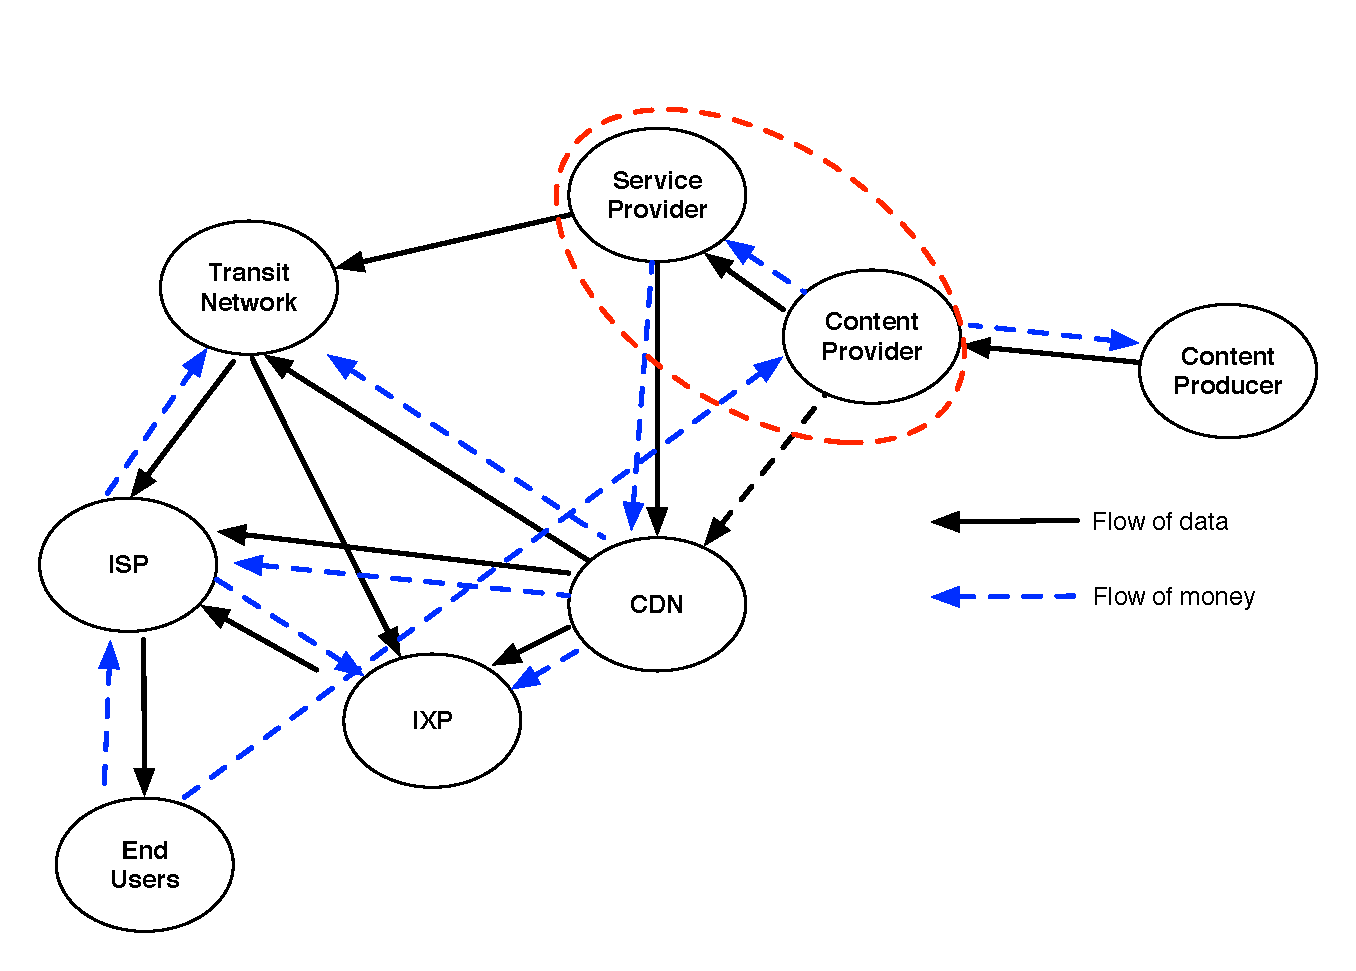
\includegraphics[scale=0.4]{graphs/business-relationship.eps}
\end{center}
\caption{Complex relationship of entities in Internet.
The data flow from content producer to content provider. 
Content producer such as movies companies send their movies to content provider for example: Netflix and Hulu.
Content providers then deliver the movies using CDN or they also can use their upstream provider.
Depends on routing and peering policy, data from CDN can flow directly to ISP or flow to ISP via IXP (Internet Exchange) or via transit network. 
Flow of data noted by straight arrow and flow of money noted by dash arrow line.
In current modern Internet topology, content provider and service provider can be merged in on entity, for example: Google.
Labovitz et al.,\cite{Labovitz:2010:IIT:2043164.1851194} mentioned that the hyper-giant entities such as Google doing massive peering to IXP in order to be closed to ISP. 
Although CDN is placed close to ISP network, it does not guarantee end-users can get good quality video stream \cite{Krishnan:2009:MBE:1644893.1644917}.
Other than technical complexity as mentioned before, CDN also faces economic complexity\cite{dispute}.
Therefore, the future of CDN business is likely to live deeper into ISP networks, more integrated into and interleaved with ISP infrastructures.}
\label{fig:businessrelationship}
\vspace{-2mm}
\end{figure} 

\begin{figure}[hb]
\begin{center}
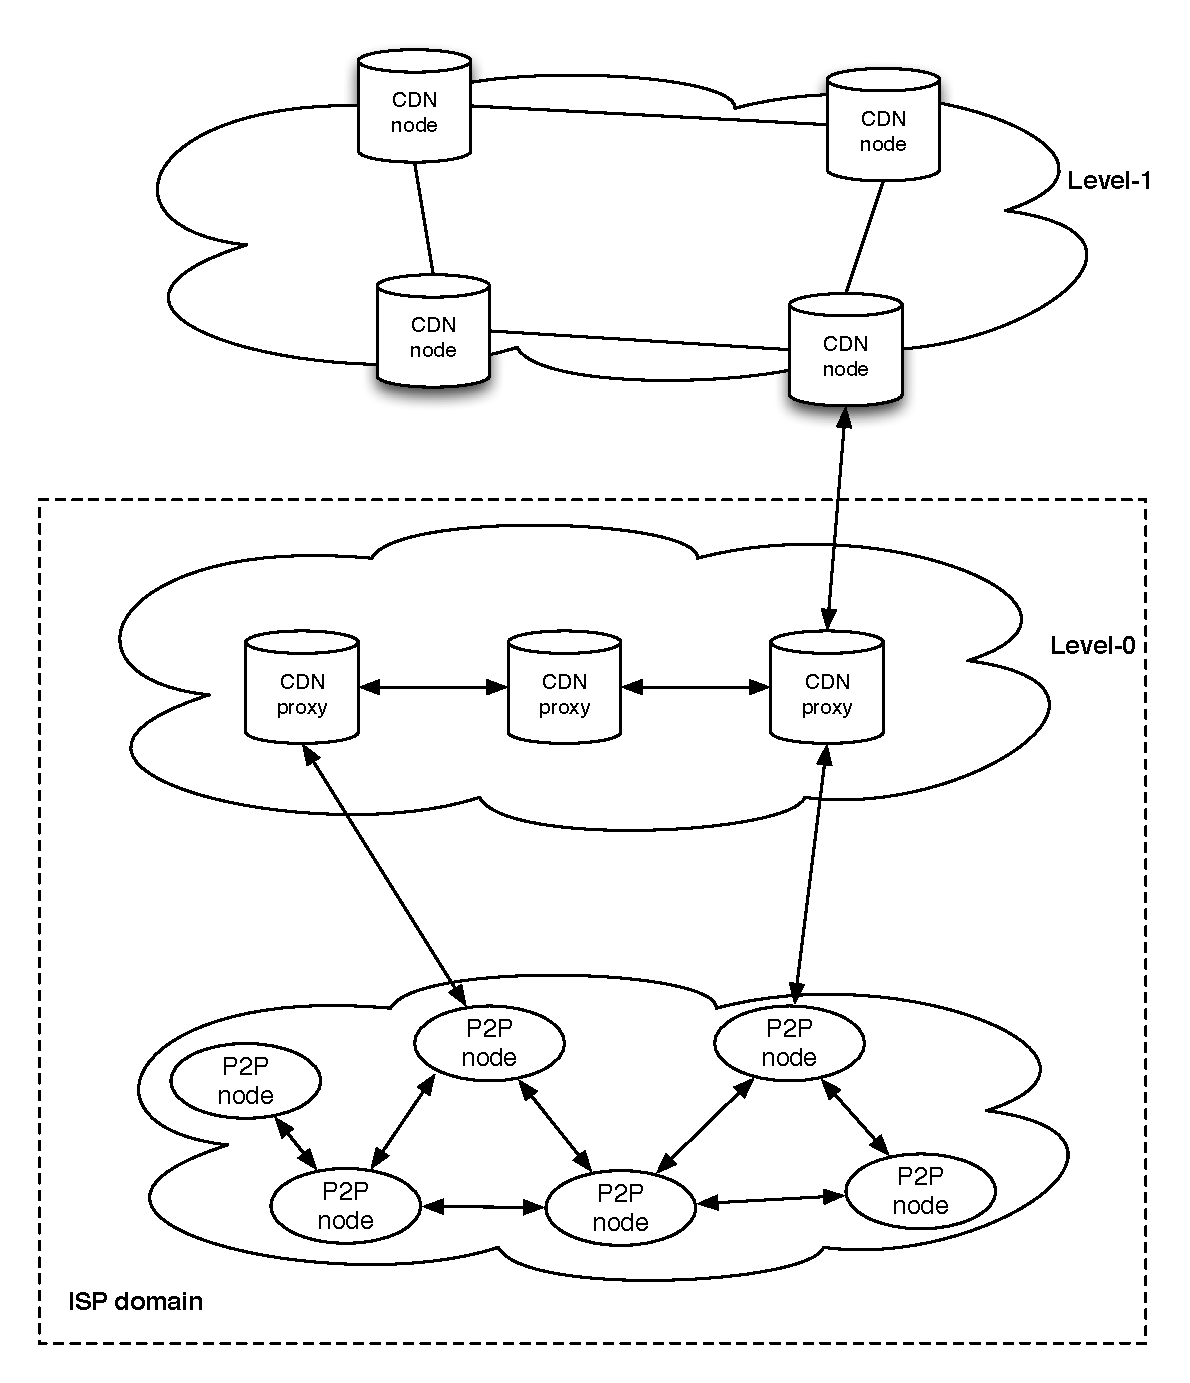
\includegraphics[scale=0.4]{graphs/two-tier-cdn-topology.eps}
\end{center}
\caption{Two tier CDN-P2P topology.
The CDN proxy maintained by ISP. ISP also has CDN node. CDN node can exchange contents with other CDN node owned by other CDN companies.P2P nodes are ISP's customers that run P2P software.}
\label{fig:twotier}
\vspace{-2mm}
\end{figure} 


 
%%%%%%%%%%%%%%%% %%%%%% SYSTEM DESCRIPTION %%%%%%%%%%%%%%%%%%%%%%%
\section{System Description}\label{description}

Figure \ref{fig:twotier} shows our system architecture model,
consisting of a two-level CDN (Level-1 and Level-0), and a P2P network.
This two-level CDN follows the hierarchical model in Maki et
al.\cite{NaoyaMAKI2012}, with some modifications.
The Level-1 CDN consists of high capacity servers strategically placed to increase network backbone capacity.
The Level-1 CDN is similar to current CDN networks, where CDN nodes
can communicate with each other by using a common interconnect interface even though the CDN nodes are owned by different companies or different ISPs \cite{cdni}.
The Level-0 CDN consists of CDN proxies owned or managed by an ISP and placed close to end users.
The CDN proxies join the P2P network along with other nodes owned by the end users.

The proxies communicate with each other to serve content requests from the users, serving the contents from their caches if the content is available 
or retrieving it from the Level-1 CDN servers otherwise.
Some end user nodes assist the proxies to serve content requests by
uploading the contents in their caches to other end user nodes, and a
user node may either receive content exclusively from the proxies or
from both the proxies and other user nodes, hence creating a P2P swarm.
The user nodes are configured to not communicate with nodes outside
the ISP's network, limiting the P2P swarm to a single ISP (or an administrative domain).

In this P2P network, the proxies can be considered to be super nodes,
or super seeders, which serve all contents that cannot be served by
other nodes.  The proxies also coordinate the user nodes, whether they
act as seeders or leechers.  The proxies should satisfy all users
while minimizing their resource usage, e.g., bandwidth and cache
capacity, by optimizing the utilization of seeders in the P2P swarm.
In the case of file sharing, the proxies may not need to serve
contents to the seeders if the upload rate from the user nodes in the
P2P swarm is enough to satisfy all users.  In the case of streaming
content, the proxies serve the contents at the full streaming rate to
the seeders; the leechers do not need to receive the full rate from
the proxies as they also receive some content from the seeders.  Also
in this case, even though the upload rate from the user nodes in the
P2P swarm is enough, relying only on user nodes may cause some nodes
to experience high latency, hence the proxies should have a good
coordination strategy to satisfy the latency requirements.

The aim in introducing this system is cost reduction for the ISP, by
reducing its core network needs and data volume with its own upstream
provider, and its costs when providing its own CDN.  Thus, the ISP may
offer incentives, e.g., a subscription fee discount, to its users in
order to get them to participate in the P2P swarm.  It should also
devise a strategy for its offers in order to achieve its commercial
objectives, including customer satisfaction.  The next section
analyzes this system and the strategies of an ISP in introducing this
system.

  
 
%%%%%%%%%% SYSTEM MODEL %%%%%%%%%%%%%%%%%%%%%%%%%%%
\section{System Model and Analysis}\label{systemmodel}

We present a model for the interaction between P2P and CDN using a
simple, single bitrate for video streaming as shown in
Fig.\ref{fig:twotier2}.  The model is a stochastic fluid model similar
to \cite{4215694}.  While the authors in \cite{4215694} focus on the
probability of degraded service on small and large systems, our work
focuses on finding the minimum capacity for a CDN proxy to support the
system.  Minimum capacity is very important for capacity planning.  In
the next subsection we also present a simple game theory model to
describe the interaction between the ISP who operates the P2P-CDN and
the users.  We aim to find out the indifferent utility function
between ISP and users.

\begin{figure}[tb] 
\begin{center}
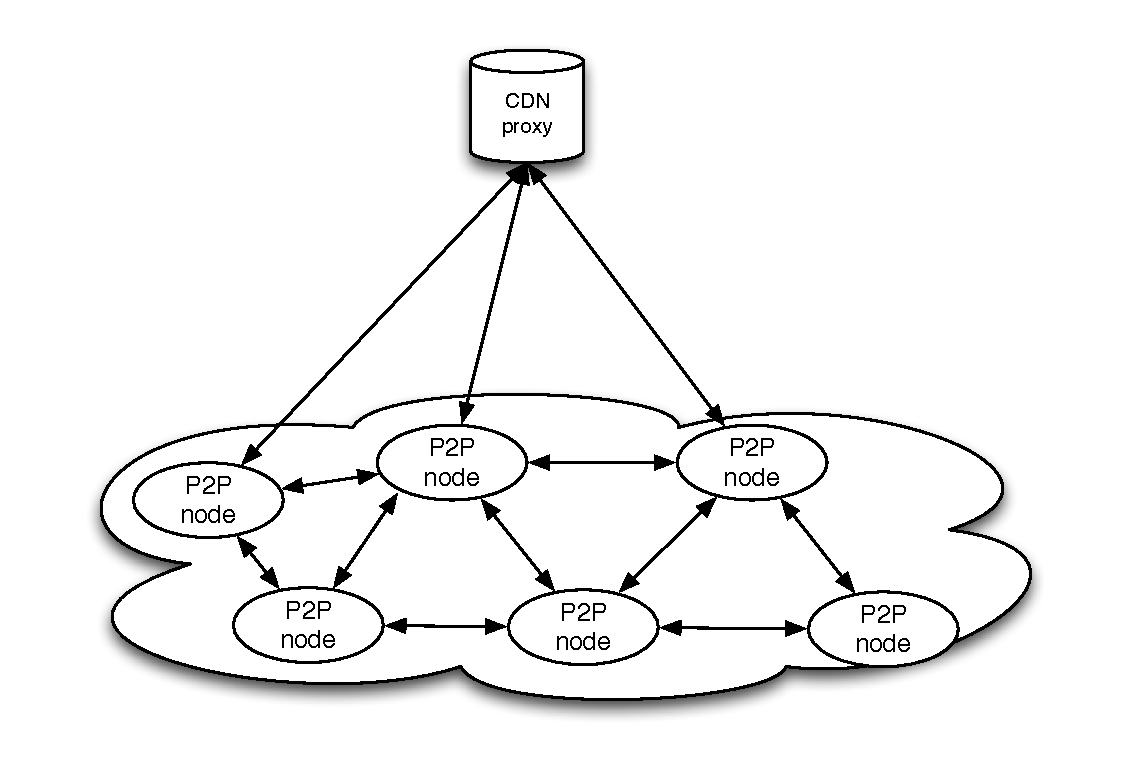
\includegraphics[scale=0.4]{graphs/two-tier-cdn-topology-2.eps}
\end{center}
\caption{System architecture on L0. P2P nodes that run on user home gateway communicates to CDN proxy.}
\label{fig:twotier2}
\vspace{-2mm}
\end{figure}

\subsection{System in Stationary State}

Let the number of leechers and the number of seeders in the P2P swarm,
not including the CDN proxy, be $n_l$ and $n_s$, and the bitrate $r$.
In order to satisfy the users' requests for streaming content, the
minimum total upload bitrate to the P2P swarm is $(n_s + n_l)r$.  Let
the upload capacity of each seeder be $u_s$, $0 \leq u_s \leq 1$,
therefore the minimum CDN proxy capacity to support the system is:
\begin{equation}
        U_p = n_sr + n_lr - min(n_su_sr, n_lr).
\end{equation}
Note that if $n_lr$ is less than the upload capacity of the seeders, the proxy does not need to serve the leechers.
Also note that if the system is for file sharing, then the CDN proxy does not need to serve the seeders.
From the above equation, we define $X=\frac{n_l}{n_s}$, which is the ratio of the number of leechers to the number of seeders, and we normalize $r=1$, hence:
\begin{equation}
        \frac{U_p}{n_s} = (1 + X - min (u_s,X)),
\end{equation}
which means that the upload capacity requirement of the CDN proxy relative to the number of seeders will be higher as $X$ increases beyond $X = u_s$.

\begin{figure}[hb] 
\begin{center}
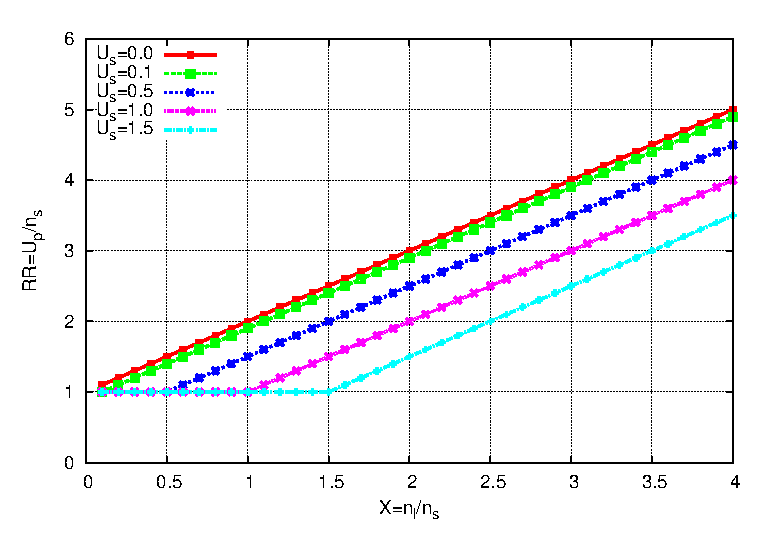
\includegraphics[scale=0.5]{graphs/stable-steady-state.eps}
\end{center}
\caption{Steady-state requirement for upload capacity relative to the
  number of seeders.}
\label{fig:steadystate}
\vspace{-2mm}
\end{figure}

Figure \ref{fig:steadystate} shows the system at equilibrium.
For $u_s=1.5$, the minimum required capacity CDN proxy relative to the number of seeders to support the system can be achieved if the ratio of leechers to seeders is less than $1.5$.
We see that the CDN proxy prefers a higher $u_s$ in the system.
A special case is $u_s = 0$, which is equivalent to no P2P swarm.
It is also clear that as $X$ increases, the CDN proxy must add capacity, thus adding the cost for the ISP.

\begin{figure*}[thb]
\begin{minipage}[b]{0.4\linewidth}
\centering
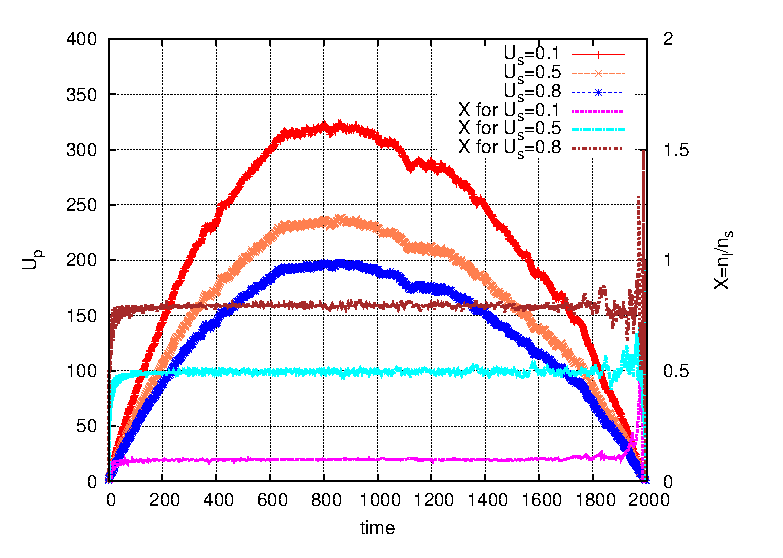
\includegraphics[width=2.8in]{graphs/U_p_n_1000.eps}
\caption{$U_p$ for $N=1000$ for admission policy 1.}
\label{fig:U_p_1000_1}
\end{minipage}
\hspace{0.5cm}
\begin{minipage}[b]{0.5\linewidth}
\centering
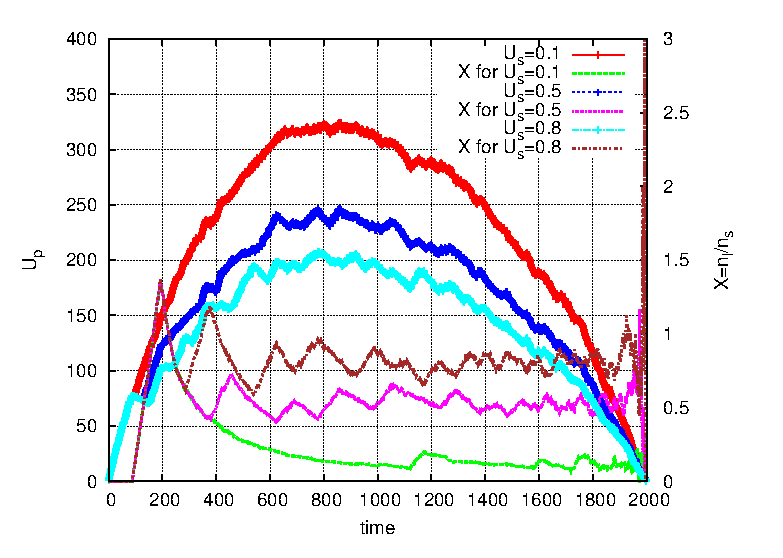
\includegraphics[width=2.8in]{graphs/U_p_n_1000_admi.eps}
\caption{$U_p$ for $N=1000$ for admission policy 2.}
\label{fig:U_p_1000_2}
\end{minipage}
\end{figure*}

\subsection{System with Churn}\label{sec:stablesystemwithchurn}

In this analysis, we assume peers (user nodes) join at random times, stay in the system for random periods of time, then leave.
We assume the peer arrivals follow a Poisson process with rate $\lambda$, and peers staying in the system follow a general probability distribution with mean $\frac{1}{\gamma}$.
Let $N(t)$ be the number of peers in the system at time $t$, i.e., the
number of nodes in a $M/G/\infty$ queue.  We can denote $U_p$ as a function of time $t$
\begin{equation}
        U_p(t) = N(t)r - min(n_s(t) u_s r, (N(t) - n_s(t))r),
\end{equation}
where $N(t) = n_s(t) + n_l(t)$, and $n_s(t)$ is determined by the system's admission policy.

%%% rdv why you chose these two candidates is totally unclear.
We now compare two admission policies:
1. The system starts admitting new arrivals as seeders until $(n_su_s > n_l)$, then each arrival is admitted as a seeder or a leecher according to the equation.     
2. The system admits arrivals every $d$ time interval. If $(n_su_s > n_l)$ at the beginning of a time interval, all arrivals within the time interval are admitted as leechers, otherwise as seeders.

Figure \ref{fig:U_p_1000_1} shows the $U_p$ values during simulation
with $N=1000, \lambda=2, \mu=2, u_s=\{0.1, 0.5, 0.8\}$, and we use the
first admission policy in this simulation.  We also plot ratio values
$X$ using the scale on the right.  Figure \ref{fig:U_p_1000_2} shows
the $U_p$ values during simulation using the second admission policy
with $delta_t=1.0$ and other parameters kept unchanged.  From both
figures, we can see that the first admission policy can stabilize the
value $X$ in order to keep the CDN proxy capacity high enough to
supply the system.  In the second admission policy, the CDN proxy
decides the same role for all peers arriving in a time interval.
Figure \ref{fig:cdf} shows the CDF of $X$ for $U_s=0.1, U_s=0.5,
\text{and } U_s=0.8$ for both admission policies.  We can see that the
second admission policy gives a higher variance, while the first
admission policy can keep the ratio ideal.  Finally, we can see that
seeder upload makes a good contribution to this system.  The next
section discusses how to give incentives to the peers in this system.

\begin{figure}[hb] 
\begin{center}
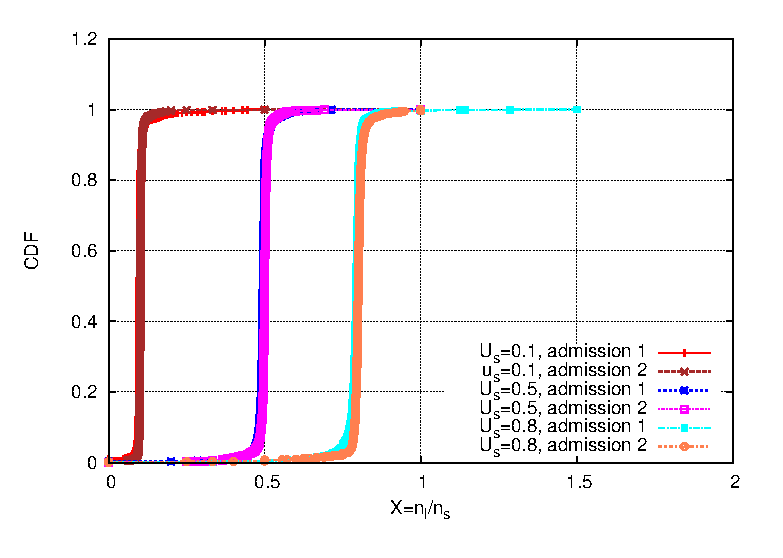
\includegraphics[scale=0.6]{graphs/cdf.eps}
\end{center}
\caption{CDF of $n_l/n_s$. We can see that the variance is higher for admission policy 2 compared to the admission policy 1.}
\label{fig:cdf}
\vspace{-2mm}
\end{figure}
 
\subsection{ISP Strategies: Game Theory Approach}

In this section, we present a simple game theory approach for analysis
of ISP strategies.  Game theory is a mathematical framework for
analyzing situations where decisions are made by a set of two or more
rational players~ \cite{gametheory}.  The basic elements of a game
are: rational players, strategies, and a payoff or utility function.
Rational players choose a strategy for maximizing their payoff.  An
extensive-form game is a representation of the corresponding decision
nodes in a directed tree.  Later, we will use an extensive-form game
to represent our game.  In our model, the ISP has already attempted to
implement a solution for peer-assisted CDN.  Moreover, it is
reasonable to assume that the ISP is naturally an initiator.  A
Stackelberg game, also known as a leader-follower game, is a class of
game where one player, the leader, initiates the decision making and
where the second player, the follower, responds to the actions by the
leader.  In our model, the ISP can be modeled as a leader who decides
to implement peer-assisted or not according to its expected payoff,
while users can be modeled as followers that evaluate the decision of
the ISP and respond according to their available actions and payoffs.
In this section, we will focus on the ISP side.

\newtheorem{theorem}{Definition}
\begin{theorem}[ISP Strategies]
We define the pure strategy space $S_{isp}$ to include two strategies, $s \in \{CDN, CDN-P2P\}$ and corresponding subscription fees $P^{s}$.
Futhermore, we denote the strategies as:
\begin{itemize}
	\item $s_1 = (CDN, P^{s_1})$ : the ISP decides to use CDN only and thus keeps charging the initial subscription free $P^{s_1}$.
	\item $s_2 = (CDN-P2P, P^{s_2})$ : the ISP decides recommends peer-assisted and offers a subscription fee $P^{s_2} \le P^{s_1}$.
\end{itemize}
Where the ISP strategy space $S_{isp} = \{s_1,s_2\}$.
\end{theorem}

\begin{figure}[tb] 
\begin{center}
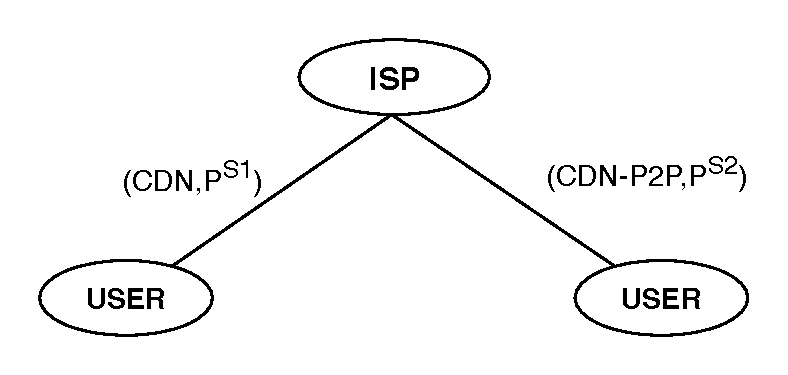
\includegraphics[scale=0.5]{graphs/game-tree-2.eps}
\end{center}
\caption{Extensive form of game between ISP's strategies}
\label{fig:gametree}
\vspace{-2mm}
\end{figure}

\subsubsection{ISP Payoff}

We now describe the payoff function for the ISP in our model.  
We assume a profit maximizing ISP that gains higher utility in proportion to the increasing profit, which is only determined by the revenue from users and the bandwidth cost to reach the users.

For the revenue model, we assume that the ISP collects revenue solely
by charging an initial flat rate subscription fee $P^{(s_1)}$ to its
$N$ number of users who purchase Internet access with equal and fixed
quality of service.  ISPs are often price discriminatory towards their
customers and thus operate with different price levels for different
bandwidth or QoS.  The also often get revenue from other businesses
such as email hosting, web hosting, etc.  In our model, we do not
include such revenue, and we found it reasonable only to focus on
users that buy the same Internet access product.  Given the above
simplifications, the ISP collects a total revenue (when deciding on a
strategy $s$) of $R = N P^{(s)}$.  The analysis focuses on the ISP
side only, and we are very interested to see the difference ($\delta$)
between payoff of strategy $s_1$ and strategy $s_2$.  For strategy
$s_1$, the payoff for the ISP is:
\begin{eqnarray}
	\pi^{(s_1)}_{(N)}&=&\pi^{(s_1)}_{(n_s)}\\
	&=&n_l P^{(s_1)} - n_l T P_t
\end{eqnarray}
note that in strategy $s_1$ we assume all peers get their requested
stream from the, CDN thus all peers are seeders.

For strategy $s_2$, the ISP has payoff:
\begin{eqnarray}
	\pi^{(s_2)}_{(N)} &=& \pi^{(s_2)}_{(n_l)} + \pi^{(s_2)}_{(n_s)}\\
	\nonumber &=&n_l p^{(s_1)} - n_lTP_t + max (n_s u_s,n_l)T P_t\\
	&+&n_s P^{(s_2)} - n_s T P_t
\end{eqnarray}
note that in $n_l p^{(s_1)}$ we use $p^{(s_1)}$ because leechers do
not join the peer-assisted mode offered by the ISP, thus the price is without discount.

Therefore payoff difference between strategy $s_1$ and $s_2$ is:
\begin{eqnarray}
	\delta &=& n_l P^{(s_1)} - n_l T P_t \\
	&-& n_l p^{(s_1)} - n_lTP_t + max (n_s u_s,n_l)T P_t \\
	&+& n_s P^{(s_2)} - n_s T P_t
\end{eqnarray}

Our notation is as follows:
\begin{itemize}
	\item $n_s$ is the number of seeders.
	\item $n_l$ is the number of leechers.
	\item $P^{(s_1)}$ is the subscription fee for strategy $s_1$
	\item $P^{(s_2)}$ is the discounted subscription fee for strategy $s_2$.
	\item $T$ is the video (streaming) traffic bitrate. 
	\item $P_t$ is the transport cost. 
	\item $U_s$ is the upload rate of seeders.
	\item $\tau^{s_1}$ is the traffic cost for strategy $s^{(s_1)}$.
	\item $\tau^{s_2}$ is the traffic cost for strategy $s^{(s_2)}$.
\end{itemize}
Explanation of notation as follows:
$n_lP^{s_1}$ is ISP revenue and $\text{max}((TP_tn_l - n_su_sTP_t),0)$ is ISP traffic cost.

%%% rdv I don't think these paragraphs make much sense.
The traffic cost $\pi^{(s_1)}_{(n_l|n_s)}$ depends on the threshold
value $n_l/n_s$ that we discussed in
Sec.\ref{sec:stablesystemwithchurn}.  If $n_su_s > n_l$, then the
bandwidth cost is minimized because the ISP does not need to add seeders,
so leechers can be added to the system instead.  If $n_su_s < n_l$, then
the bandwidth cost is maximized because the ISP needs to add seeders.  The
maximum difference between these values and 0 is the cost of ISP
traffic.  We also note that $P^{(s_2)}$ is the price that the ISP gives in
strategy $s_2$.  $P^{(s_2)}$ is the discount price because users accept
strategy $s_2$ to join the peer-assisted CDN.  We can get the discount price
by indifference payoff between strategy $s_1$ and $s_2$ with total
peer $N$:
\begin{eqnarray}  
	\pi^{(s_1)}_{(N)} &=& \pi^{(s_2)}_{(N)}\\
	N.P^{(s_1)} - \tau^{(s_1)} &=& N.P^{(s_2)} - \tau^{(s_2)}\\
	P^{(s_2)} &=& P^{(s_1)} - \frac{1}{N} (\tau^{(s_1)} -  \tau^{(s_2)} ) 
\end{eqnarray}
Where $\tau^{(s_2)}=n_sTP_t$ is the traffic cost for strategy $s_2$.
The factor $\frac{1}{N} (\tau^{(s_1)} - \tau^{(s_2)} )$ is the
discount.  We can define the discount factor as $\frac{\gamma}{N}
(\tau^{(s_1)} - \tau^{(s_2)} )$.  Maximum discount that ISP can give
to user when $\gamma=1$ and minimum discount that ISP can give to user
when $\gamma=0$.  We can also say that $\gamma$ is a ratio that
express how much of the ISP expected utility increase it wants to
share with its users.

\begin{figure}[thb] 
\begin{center}
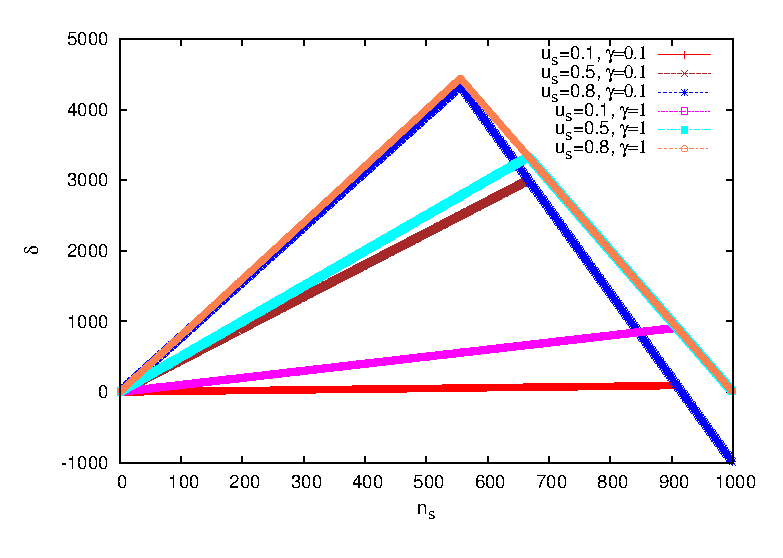
\includegraphics[scale=0.65]{graphs/plotpay.eps}
\end{center}
\caption{$\delta$ between strategy $s_1$ and $s_2$ with $U_s$ variation and $\gamma$ variation.The intersection of lines with x-axis = 0 is the point where ISP has minimum payoff with maximum number of seeders. }
\label{fig:delta}
\vspace{-2mm}
 \end{figure}
 
\subsubsection{Numerical Result}

In this subsection we numerically evaluate the ISP strategy.
The assumptions that we use for this numerical simulation are:
\begin{itemize}
	\item We assume that all traffic is video traffic.
	\item We assume that user utilizes $100\%$ of his/her Internet connection capacity.  
	\item We assume that users never turn off their gateways, so the ISP do not need to penalize users.
	\item We assume there is no investment cost, though the ISP may
          need to give different firmware software to run
          peer-assisted application inside users home gateway. We
          assume that cost is very small, thus we assume investment
          cost is zero.
\end{itemize}
The parameter values that we use in this numerical simulation are as follows:
\begin{table}[hb]%[tb]
\caption{Parameters values for simulation}
\label{table:1}
\begin{center}
\begin{tabular}{c|c}
\hline
$u_s$ & $\{0.1, 0.5, 0.8\}$ \\
\hline
$N$ & $1000$\\
\hline
$T$ & $1$Mbps \\
\hline
$P_t$ & $10$USD \\
\hline
$P^{(s_1)}$ & $50$USD\\
\hline
$\gamma$ & $\{0.1,1.0\}$ \\
\hline
\end{tabular}
\end{center}
\end{table}

Figure \ref{fig:delta} shows the difference payoff between strategy $s_1$ and $s_2$.
The intersection between the lines and x-axis=0 is the point where ISP
has the minimum payoff with the maximum number of seeders.
for $u_s=0.1, \gamma=0.1$, the maximum number of seeders is 449.  
for $u_s=0.1, \gamma=1$, the maximum number of seeders is 450. 
for $u_s=0.5, \gamma=0.1$, the maximum number of seeders is 469.  
for $u_s=0.5, \gamma=1$, the maximum number of seeders is 471. 
for $u_s=0.8, \gamma=0.1$, the maximum number of seeders is 484.  
for $u_s=0.8, \gamma=1$, the maximum number of seeders is 488.
 if we compare same $\gamma$ for different values of $u_s$, the
 different number of minimum seeders is large.  
If we compare the same $u_s$ for different $\gamma$, then the different minimum seeders is small.   
Therefore, we can see that the $u_s$ factor is dominant over the $\gamma$ factor. 



%%%%%%%%%%%%%%%%% RELATED WORK %%%%%%%%%%%%%%%%%%%%%%%%
\section{Related Work} 

Content Distribution Networks with peer assist have been successfully
deployed on the Internet, such as Akamai
\cite{Huang:2008:UHC:1496046.1496064} and LiveSky
\cite{Yin:2010:LEC:1823746.1823750}.  The authors of
\cite{Huang:2008:UHC:1496046.1496064} conclude from two real world
traces that hybrid CDN-P2P can significantly reduce the cost of
content distribution and can scale to cope with the exponential growth
of Internet video content.  Yin et
al. \cite{Yin:2010:LEC:1823746.1823750} described commercial operation
of a peer-assisted CDN in China.  LiveSky solved several challenges in
the system design, such as dynamic resource scaling of P2P, low
startup latency, ease of P2P integration with the existing CDN
infrastructure, and network friendliness and upload fairness in the
P2P operation.  Xu et al.\cite{DBLP:journals/corr/abs-1212-4915}
using game theory, showed that the right cooperative profit
distribution of P2P can help the ISP to maximize the utility.  Their
model can easily be implemented in the context of current Internet
economic settlements.  Misra et
al.\cite{Misra:2010:IPS:1811099.1811064} also mentioned the
importance of P2P architecture to support content delivery networks.
The authors use cooperative game theory to formulate simple
compensation rules for users who run P2P to support content delivery
networks.

The idea of telco- or ISP-managed CDN has been proposed in recent
years.  The complexity of the CDN business encourage telcos and ISPs
to manage their own CDN, rather than allow others to run CDNs on their
networks.  It has been shown that it is cost effective
\cite{federation}\cite{norton2011internet}.  Kamiyama et
al. \cite{NoriakiKAMIYAMA2013} proposed optimally ISP operated CDN.
Kamiyama et al. mentioned that, in order to deliver large and rich
Internet content to users, ISPs need to put their CDNs in data
centers.  The locations are limited while the storage is large, making
this solution effective, using optimum placement algorithm based on
real ISP network topologies.  The authors found that inserting a CDN
into an ISP's ladder-type network is effective in reducing the hop
count, thus reduce total link cost.  Cisco has initiated an effort to
connect telco- or ISP-managed CDNs to each other, to form a CDN
federation \cite{federation} using open standards \cite{cdni}.  They
argue that the current CDN architecture is not close enough to the
users and ISPs can fill this position.

The idea of utilizing the user's computation power to support ISP
operation is not new.  The Figaro project \cite{figaro} proposed
residential gateway as an integrator of different networks and
services, becoming an Internet-wide distributed content management for
a proposed future Internet architecture \cite{figaro}.  Cha et
al.,\cite{Cha:2008:NTP:1855641.1855646} performed trace analysis and
found that an IPTV architecture powered by P2P can handle a much
larger number of channels, with limited demand for infrastructure
compare to IP multicast.  Jiang et al.
\cite{Jiang:2012:OMD:2413176.2413193} proposed scalable and adaptive
content replication and request routing for CDN servers located in
users' home gateways.  Maki et al.\cite{NaoyaMAKI2012} propose traffic
engineering for peer-assisted CDN to control the behavior of clients,
and present a solution for optimizing the selection of content files.
Our work is the same system model architecture, using different level
of topologies (Level-0 and Level-1).  Maki et al. use different names,
local domain and global domain.  While our work focuses on the fluid
limit for the number of peers needed to support video stream bitrate
in a single bitrate system and modeling simple economic incentives for
ISPs, Maki et al. focus on a traffic engineering algorithm for
optimizing the selection of content files and controlling the behavior
of clients.

%%%%%%%%%%%%%%%%% CONCLUSION %%%%%%%%%%%%%%%%%%%%%%%%%
\section{Conclusion and Future Work}\label{conclude}

This paper presents a scheme for a peer-assisted, ISP-managed CDN
model that estimates the lower bound of the number of peers based on a
stochastic fluid model, and estimates the economic incentive for the
ISP based on game theory.  We found that the upload rate seeder has a
big influence on the system.  This observation agrees with that of
\cite{DBLP:journals/corr/abs-1212-4915}.  Our numerical results show
that a peer-assisted CDN managed by ISP or telco is feasible to deploy
and does not harm the ISP's business.  Our future work will include
energy efficiency trade off for this peer-assisted, ISP-managed CDN.
We are very interested in knowing how much energy can be saved by the
ISP and how much the energy consumption at the user's home gateway
will increase in this architecture.



%%%%%%%%%%%%%%%%% ACKNOWLEDGEMENT %%%%%%%%%%%%%%%%%%%%%
%\section*{Acknowledgements}
%We thank Joe Touch for suggestions.


\bibliographystyle{ieicetr}% bib style
\bibliography{jurnal}% your bib database

%\begin{thebibliography}{99}% more than 9 --> 99 / less than 10 --> 9
%\bibitem{}
%\end{thebibliography}

\profile[]{Mohamad Dikshie Fauzie}{%
was born in 1976. 
He received a bachelors degree and a master's degree from Institute of Technology Bandung, Indonesia.
He is currently a Ph.D candidate at Keio University's Shonan Fujisawa Campus.
}

\profile[]{Achmad Husni Thamrin}{%
is Assistant Professor at Keio University. 
He is a graduate of Keio University, Graduate School of Media and Governance (Ph.D 2005, MMG, 2002). 
His research interests include multicast, Internet over broadcast media, and peer-to-peer networks.
}

%\profile[photos/a3.eps]{Rodney Van Meter}{%
%received a B.S. from the California Institute of Technology in 1986,
%an M.S. from the University if Southern California in 1991, and
%a Ph.D. from Keio University in 2006. His research interests include
%storage systems, networking, post Moore's law computer architecture,
%and quantum computing. He is an Associate Professor of Environment and
%Information Studies at Keio University's Shonan Fujisawa Campus.
%}
\profile[]{Jun Murai}{%
was born in March 1955 in Tokyo. Graduated Keio University in 1979,
Department of Mathematics, Faculty of Science and Technology.
He received his M.S. for Computer Science from Keio University in 1981,
and received his Ph.D. in Computer Science, Keio University in 1987. 
He specializes in computer science, computer network, and computer 
communication. He is currently Dean of the Faculty of Environment and
Information Studies, Keio University since October 2009. Former
Vice-President of Keio University from May 2005 to May 2009. He was
an Executive Director of the Keio Research Institute at SFC, Keio
University from 1999 to 2005.
}
 
\end{document}
